\hypertarget{singleton_8hpp}{
\section{include/singleton.hpp File Reference}
\label{singleton_8hpp}\index{include/singleton.hpp@{include/singleton.hpp}}
}
Implementation du design pattern singleton.  


{\tt \#include $<$iostream$>$}\par


Include dependency graph for singleton.hpp:\nopagebreak
\begin{figure}[H]
\begin{center}
\leavevmode
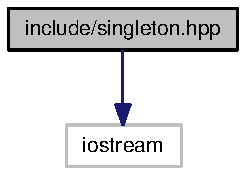
\includegraphics[width=77pt]{singleton_8hpp__incl}
\end{center}
\end{figure}
\subsection*{Classes}
\begin{CompactItemize}
\item 
class \hyperlink{classSingleton}{Singleton$<$ T $>$}
\begin{CompactList}\small\item\em Template de classe permettant de rendre une classe instanciable une seule fois. \item\end{CompactList}\end{CompactItemize}


\subsection{Detailed Description}
Implementation du design pattern singleton. 

\begin{Desc}
\item[Author:]GDD 

Arnaud Faure 

Pauline Requena \end{Desc}
\begin{Desc}
\item[Version:]0.1 \end{Desc}
\begin{Desc}
\item[Date:]29 mars 2009\end{Desc}
Implementation du design pattern singleton pour rendre une classe instanciable une unique fois. 